\documentclass[a4paper,11pt]{article}
\usepackage{amsmath,amsthm,amsfonts,amssymb,amscd,amstext,vmargin,graphics,graphicx,tabularx,multicol} 
\usepackage[francais]{babel}
\usepackage[utf8]{inputenc}  
\usepackage[T1]{fontenc} 
\usepackage{pstricks-add,tikz,tkz-tab,variations}
\usepackage[autolanguage,np]{numprint} 

\setmarginsrb{1.5cm}{0.5cm}{1cm}{0.5cm}{0cm}{0cm}{0cm}{0cm} %Gauche, haut, droite, haut
\newcounter{numexo}
\newcommand{\exo}[1]{\stepcounter{numexo}\noindent{\bf Exercice~\thenumexo} : \marginpar{\hfill /#1}}
\reversemarginpar


\newcounter{enumtabi}
\newcounter{enumtaba}
\newcommand{\q}{\stepcounter{enumtabi} \theenumtabi.  }
\newcommand{\qa}{\stepcounter{enumtaba} (\alph{enumtaba}) }
\newcommand{\initq}{\setcounter{enumtabi}{0}}
\newcommand{\initqa}{\setcounter{enumtaba}{0}}

\newcommand{\be}{\begin{enumerate}}
\newcommand{\ee}{\end{enumerate}}
\newcommand{\bi}{\begin{itemize}}
\newcommand{\ei}{\end{itemize}}
\newcommand{\bp}{\begin{pspicture*}}
\newcommand{\ep}{\end{pspicture*}}
\newcommand{\bt}{\begin{tabular}}
\newcommand{\et}{\end{tabular}}
\renewcommand{\tabularxcolumn}[1]{>{\centering}m{#1}} %(colonne m{} centrée, au lieu de p par défault) 
\newcommand{\tnl}{\tabularnewline}

\newcommand{\trait}{\noindent \rule{\linewidth}{0.2mm}}
\newcommand{\hs}[1]{\hspace{#1}}
\newcommand{\vs}[1]{\vspace{#1}}

\newcommand{\N}{\mathbb{N}}
\newcommand{\Z}{\mathbb{Z}}
\newcommand{\R}{\mathbb{R}}
\newcommand{\C}{\mathbb{C}}
\newcommand{\Dcal}{\mathcal{D}}
\newcommand{\Ccal}{\mathcal{C}}
\newcommand{\mc}{\mathcal}

\newcommand{\vect}[1]{\overrightarrow{#1}}
\newcommand{\ds}{\displaystyle}
\newcommand{\eq}{\quad \Leftrightarrow \quad}
\newcommand{\vecti}{\vec{\imath}}
\newcommand{\vectj}{\vec{\jmath}}
\newcommand{\Oij}{(O;\vec{\imath}, \vec{\jmath})}
\newcommand{\OIJ}{(O;I,J)}


\newcommand{\reponse}[1][1]{%
\multido{}{#1}{\makebox[\linewidth]{\rule[0pt]{0pt}{20pt}\dotfill}
}}

\newcommand{\titre}[5] 
% #1: titre #2: haut gauche #3: bas gauche #4: haut droite #5: bas droite
{
\noindent #2 \hfill #4 \\
#3 \hfill #5

\vspace{-1.6cm}

\begin{center}\rule{6cm}{0.5mm}\end{center}
\vspace{0.2cm}
\begin{center}{\large{\textbf{#1}}}\end{center}
\begin{center}\rule{6cm}{0.5mm}\end{center}
}



\begin{document}
\pagestyle{empty}
\titre{{\Large Le petit truc en plus : le code barre !}}{Nom :}{Prénom :}{5ème}{}


\vspace*{1cm}



\textit{\textbf{{\large A rendre avant le  17 septembre !}}}\\

\begin{flushright}
\fbox{{\LARGE \textbf{NOTE} : . . . /5}  }
\end{flushright}

\vspace*{1cm}

Dans le commerce, chaque produit est identifié par un nombre à 13 chiffres.\\
Le 13ème est une clé de contrôle : pour l'obtenir, on multiplie chaque chiffre alter-nativement par 1 puis par 3 en considérant les chiffres de gauche à droite (sans le 13ème) puis on effectue la somme de ces produits.\\
\textbf{ La clé} est alors donnée par le nombre à ajouter pour obtenir le plus petit multiple de 10.
 
  \begin{center}
  
\includegraphics[scale=1]{codebarre1.eps} 
  \end{center}
 
 Avec le numéro du code-barre ci-dessus, la somme :
 
\begin{flushleft}
 \includegraphics[scale=0.8]{codebarre2.eps} 
\end{flushleft}
 
 donne 121, d'où la clé \fbox{\textbf{9}} pour obtenir 130.\\
 
 \vspace*{1cm}
 
\textbf{ {\Large QUESTIONS :}}\\ 
 \qa Découper et coller le code-barres d'un produit de la vie courante.\\
\qa Vérifier, en précisant les calculs, la clé de contrôle de ce code-barres.\\
\qa Lorsque les 2 premiers chiffres forment un nombre compris entre 30 et 37, la société propriétaire du code est française; est-ce le cas pour le code-barres que vous avez collé ?\\

\end{document}
